% ============================================================
\chapter{Simplicial Complexes and Homology}
\label{ch:simplicial}
% ============================================================

How do you count the holes in a shape? The question sounds almost childish, yet it took some of the greatest minds in mathematics---Euler, Riemann, Poincar\'e, Emmy Noether---to arrive at a satisfying answer. The key idea, developed by Henri Poincar\'e in his landmark \emph{Analysis Situs} (1895), is to decompose a space into simple building blocks---points, edges, triangles, tetrahedra---and then use algebra to detect which combinations of these blocks form ``cycles'' that do not bound anything. Each such cycle witnesses a hole.

This is the programme of \emph{simplicial homology}: build a combinatorial skeleton of your space (a simplicial complex), define boundary operators that encode how pieces fit together, and compute the quotient ``cycles modulo boundaries.'' The resulting homology groups are topological invariants---they do not depend on the particular triangulation chosen. For topological data analysis, this machinery is indispensable: it is the engine that detects connected components, loops, cavities, and higher-dimensional voids in point cloud data.

\begin{intuition}
Simplicial complexes are the building blocks of TDA: they generalize
graphs to higher dimensions. Homology is the algebraic tool that allows
us to count the holes of each dimension in these complexes.
\end{intuition}

% ============================================================
\section{Simplices}
% ============================================================

\begin{definition}[Geometric Simplex]
A \emph{geometric $p$-simplex} is the convex hull of $p+1$
\emph{affinely independent} points $v_0, \ldots, v_p \in \R^d$:
\[
  \sigma = [v_0, \ldots, v_p]
  = \left\{ \sum_{i=0}^{p} \lambda_i v_i
    \;\middle|\;
    \lambda_i \geq 0,\; \sum_{i=0}^{p} \lambda_i = 1 \right\}.
\]
The integer $p$ is the \emph{dimension} of $\sigma$.
\end{definition}

\begin{example}
\begin{itemize}
  \item $0$-simplex: a point (vertex).
  \item $1$-simplex: a segment (edge).
  \item $2$-simplex: a triangle (filled).
  \item $3$-simplex: a tetrahedron (filled).
\end{itemize}
\end{example}

\begin{center}
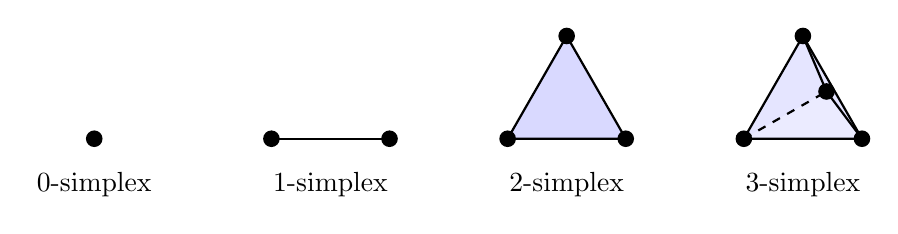
\begin{tikzpicture}[scale=1.5]
  % 0-simplex
  \fill (0,0) circle (2pt);
  \node[below] at (0,-0.2) {$0$-simplex};
  % 1-simplex
  \draw[thick] (1.5,0) -- (2.5,0);
  \fill (1.5,0) circle (2pt);
  \fill (2.5,0) circle (2pt);
  \node[below] at (2,-0.2) {$1$-simplex};
  % 2-simplex
  \fill[blue!15] (3.5,0) -- (4.5,0) -- (4,0.87) -- cycle;
  \draw[thick] (3.5,0) -- (4.5,0) -- (4,0.87) -- cycle;
  \fill (3.5,0) circle (2pt);
  \fill (4.5,0) circle (2pt);
  \fill (4,0.87) circle (2pt);
  \node[below] at (4,-0.2) {$2$-simplex};
  % 3-simplex
  \fill[blue!10] (5.5,0) -- (6.5,0) -- (6,0.87) -- cycle;
  \fill[blue!8] (5.5,0) -- (6.5,0) -- (6.2,0.4) -- cycle;
  \draw[thick] (5.5,0) -- (6.5,0) -- (6,0.87) -- cycle;
  \draw[thick,dashed] (5.5,0) -- (6.2,0.4);
  \draw[thick] (6.5,0) -- (6.2,0.4);
  \draw[thick] (6,0.87) -- (6.2,0.4);
  \fill (5.5,0) circle (2pt);
  \fill (6.5,0) circle (2pt);
  \fill (6,0.87) circle (2pt);
  \fill (6.2,0.4) circle (2pt);
  \node[below] at (6,-0.2) {$3$-simplex};
\end{tikzpicture}
\end{center}

\begin{definition}[Face]
A \emph{face} of a $p$-simplex $\sigma = [v_0, \ldots, v_p]$ is any
simplex obtained by removing one or more vertices. The \emph{$i$-th
opposite face} is:
\[
  d_i \sigma = [v_0, \ldots, \hat{v}_i, \ldots, v_p]
\]
where $\hat{v}_i$ indicates omission of vertex $v_i$.
\end{definition}

% ============================================================
\section{Abstract Simplicial Complexes}
% ============================================================

\begin{definition}[Abstract Simplicial Complex]
An \emph{abstract simplicial complex} is a pair $K = (V, \Sigma)$ where
$V$ is a finite set of vertices and $\Sigma \subseteq 2^V$ is a
collection of non-empty subsets of $V$ such that:
\begin{enumerate}
  \item For every $v \in V$, $\{v\} \in \Sigma$.
  \item If $\sigma \in \Sigma$ and $\tau \subseteq \sigma$ with
        $\tau \neq \emptyset$, then $\tau \in \Sigma$.
\end{enumerate}
Elements of $\Sigma$ are called \emph{simplices} and condition~(2) is
the \emph{closure under faces} property.
\end{definition}

\begin{definition}[Dimension]
The \emph{dimension} of a simplex $\sigma$ is
$\dim \sigma = \abs{\sigma} - 1$. The \emph{dimension} of the complex
is $\dim K = \max_{\sigma \in \Sigma} \dim \sigma$.
\end{definition}

\begin{example}
Consider $V = \{a, b, c, d\}$ and:
\[
  \Sigma = \big\{
    \{a\}, \{b\}, \{c\}, \{d\},
    \{a,b\}, \{b,c\}, \{a,c\}, \{c,d\},
    \{a,b,c\}
  \big\}.
\]
This is a simplicial complex of dimension~$2$. It contains one
$2$-simplex $\{a,b,c\}$ (filled triangle), four $1$-simplices (edges),
and four $0$-simplices (vertices).
\end{example}

% ============================================================
\section{Chains, Boundaries, and Cycles}
% ============================================================

Fix a field $\mathbb{F}$ (typically $\mathbb{F}_2 = \Z / 2\Z$).

\begin{definition}[Chain Group]
The \emph{group of $p$-chains} of $K$ with coefficients in $\mathbb{F}$
is the vector space:
\[
  C_p(K; \mathbb{F}) = \bigoplus_{\sigma \in \Sigma,\, \dim \sigma = p}
  \mathbb{F} \cdot \sigma.
\]
An element of $C_p$ is a formal linear combination of $p$-simplices.
\end{definition}

\begin{definition}[Boundary Operator]
The \emph{boundary operator} $\partial_p : C_p(K) \to C_{p-1}(K)$ is
defined on generators by:
\[
  \partial_p [v_0, \ldots, v_p]
  = \sum_{i=0}^{p} (-1)^i [v_0, \ldots, \hat{v}_i, \ldots, v_p].
\]
\end{definition}

\begin{keyformulas}[title=\textbf{Fundamental Property of the Boundary}]
\[
  \partial_{p-1} \circ \partial_p = 0 \quad \forall\, p.
\]
In other words, \emph{the boundary of a boundary is zero}.
\end{keyformulas}

\begin{proposition}
For all $p \geq 0$, $\partial_{p-1} \circ \partial_p = 0$.
\end{proposition}

\begin{proof}
Let $\sigma = [v_0, \ldots, v_p]$. Then:
\begin{align*}
\partial_{p-1}(\partial_p \sigma)
&= \partial_{p-1}\left(\sum_{i=0}^p (-1)^i
   [v_0,\ldots,\hat{v}_i,\ldots,v_p]\right) \\
&= \sum_{i=0}^p (-1)^i \sum_{\substack{j=0 \\ j \neq i}}^p (-1)^{j'}
   [v_0,\ldots,\hat{v}_j,\ldots,\hat{v}_i,\ldots,v_p]
\end{align*}
where $j' = j$ if $j < i$ and $j' = j-1$ if $j > i$. Each term appears
exactly twice with opposite signs, so the sum vanishes.
\end{proof}

\begin{definition}[Cycles and Boundaries]
\begin{itemize}
  \item The group of \emph{$p$-cycles} is $Z_p(K) = \ker \partial_p$.
  \item The group of \emph{$p$-boundaries} is
        $B_p(K) = \mathrm{im}\, \partial_{p+1}$.
  \item Since $\partial_p \circ \partial_{p+1} = 0$, we have
        $B_p(K) \subseteq Z_p(K)$.
\end{itemize}
\end{definition}

% ============================================================
\section{Simplicial Homology}
% ============================================================

\begin{definition}[Homology Group]
The \emph{$p$-th homology group} of $K$ with coefficients in
$\mathbb{F}$ is the quotient:
\[
  H_p(K; \mathbb{F}) = Z_p(K) / B_p(K)
  = \ker \partial_p \,/\, \mathrm{im}\, \partial_{p+1}.
\]
The \emph{$p$-th Betti number} is
$\beta_p = \dim_\mathbb{F} H_p(K; \mathbb{F})$.
\end{definition}

\begin{keyformulas}[title=\textbf{Betti Number Formula}]
\[
  \beta_p = \dim \ker \partial_p - \dim \mathrm{im}\, \partial_{p+1}
  = \mathrm{rank}(Z_p) - \mathrm{rank}(B_p).
\]
\end{keyformulas}

\begin{theorem}[Euler--Poincar\'e Characteristic]
If $K$ is a simplicial complex of dimension $d$, its \emph{Euler
characteristic} satisfies:
\[
  \chi(K) = \sum_{p=0}^{d} (-1)^p \abs{\Sigma_p}
  = \sum_{p=0}^{d} (-1)^p \beta_p
\]
where $\Sigma_p$ denotes the set of $p$-simplices of $K$.
\end{theorem}

% ============================================================
\section{Matrix Computation of Homology}
% ============================================================

In practice, homology computation reduces to linear algebra. Fix an
ordering on simplices of each dimension. The operator $\partial_p$ is
then represented by a matrix $D_p$ with entries in $\mathbb{F}$.

\begin{algorithme}[title=\textbf{Computing Betti Numbers}]
\begin{enumerate}
  \item Build the boundary matrices $D_p$ for $p = 1, \ldots, d$.
  \item Compute $r_p = \mathrm{rank}(D_p)$ (via Smith normal form or
        Gaussian elimination over $\mathbb{F}$).
  \item Betti numbers are: $\beta_p = \abs{\Sigma_p} - r_p - r_{p+1}$.
\end{enumerate}
\end{algorithme}

\begin{codeblock}[title=\textbf{Homology via Matrix Computation}]
\begin{minted}{python}
import numpy as np

def boundary_matrix(simplices_p, simplices_pm1):
    """Boundary matrix over F_2."""
    n_rows = len(simplices_pm1)
    n_cols = len(simplices_p)
    D = np.zeros((n_rows, n_cols), dtype=int)
    idx_map = {tuple(s): i for i, s in enumerate(simplices_pm1)}
    for j, sigma in enumerate(simplices_p):
        for k in range(len(sigma)):
            face = tuple(sigma[:k] + sigma[k+1:])
            if face in idx_map:
                D[idx_map[face], j] = 1  # mod 2
    return D % 2

def betti_numbers_f2(K, dim):
    """Compute beta_0, ..., beta_dim over F_2."""
    simplices_by_dim = {}
    for s in K:
        d = len(s) - 1
        simplices_by_dim.setdefault(d, []).append(sorted(s))
    bettis = []
    for p in range(dim + 1):
        sp = simplices_by_dim.get(p, [])
        if p > 0:
            D_p = boundary_matrix(sp, simplices_by_dim.get(p-1, []))
            rk_p = np.linalg.matrix_rank(D_p) if D_p.size else 0
        else:
            rk_p = 0
        sp1 = simplices_by_dim.get(p+1, [])
        if sp1:
            D_p1 = boundary_matrix(sp1, sp)
            rk_p1 = np.linalg.matrix_rank(D_p1) if D_p1.size else 0
        else:
            rk_p1 = 0
        bettis.append(len(sp) - rk_p - rk_p1)
    return bettis
\end{minted}
\end{codeblock}

% ============================================================
\section{Computation Examples}
% ============================================================

\begin{example}[Hollow Triangle]
Let $K$ be the complex formed by three vertices $\{a, b, c\}$ and three
edges $\{a,b\}, \{b,c\}, \{a,c\}$, \emph{without} the $2$-simplex
$\{a,b,c\}$.
\begin{itemize}
  \item $D_1 = \begin{pmatrix} 1 & 0 & 1 \\ 1 & 1 & 0 \\ 0 & 1 & 1 \end{pmatrix}$
        (over $\mathbb{F}_2$), rank $2$.
  \item $\beta_0 = 3 - 2 = 1$ (one connected component).
  \item $\beta_1 = 3 - 2 - 0 = 1$ (one hole --- the triangle is hollow).
\end{itemize}
\end{example}

\begin{example}[Filled Triangle]
Add the $2$-simplex $\{a,b,c\}$ to the previous complex.
$D_2$ is the column vector $(1, 1, 1)^T$ over $\mathbb{F}_2$, rank $1$.
\begin{itemize}
  \item $\beta_0 = 3 - 2 = 1$.
  \item $\beta_1 = 3 - 2 - 1 = 0$ (the hole is filled).
  \item $\beta_2 = 1 - 1 = 0$.
\end{itemize}
\end{example}

% ============================================================
\section{Relative Homology and Exact Sequences}
% ============================================================

\begin{definition}[Relative Homology]
Let $L \subseteq K$ be a subcomplex. The \emph{relative homology} is:
\[
  H_p(K, L; \mathbb{F}) = \ker(\bar{\partial}_p) / \mathrm{im}(\bar{\partial}_{p+1})
\]
where $\bar{\partial}_p$ is induced by $\partial_p$ on the quotient
$C_p(K)/C_p(L)$.
\end{definition}

\begin{theorem}[Long Exact Sequence of a Pair]
There exists a long exact sequence:
\[
  \cdots \to H_p(L) \xrightarrow{i_*} H_p(K)
  \xrightarrow{j_*} H_p(K, L)
  \xrightarrow{\partial_*} H_{p-1}(L) \to \cdots
\]
\end{theorem}

% ============================================================
\section{Homology with GUDHI}
% ============================================================

\begin{codeblock}[title=\textbf{Homology Computation with GUDHI}]
\begin{minted}{python}
import gudhi

# Build a simplicial complex
st = gudhi.SimplexTree()
st.insert([0, 1])
st.insert([1, 2])
st.insert([0, 2])
# Hollow triangle: no 2-simplex [0,1,2]

# Betti numbers
betti = st.betti_numbers()
print(f"Betti numbers: {betti}")
# Output: Betti numbers: {0: 1, 1: 1}

# Now fill the triangle
st.insert([0, 1, 2])
betti = st.betti_numbers()
print(f"Betti numbers: {betti}")
# Output: Betti numbers: {0: 1}
\end{minted}
\end{codeblock}

% ============================================================
\section{Reduced Homology and Euler Characteristic}
% ============================================================

\begin{definition}[Reduced Homology]
The \emph{reduced homology} $\tilde{H}_p(K)$ is defined by augmenting
the chain complex with the map
$\varepsilon : C_0(K) \to \mathbb{F}$,
$\varepsilon(\sum \lambda_i v_i) = \sum \lambda_i$. We have:
\[
  \tilde{H}_p(K) = \begin{cases}
    H_p(K) & \text{if } p > 0, \\
    \ker(\varepsilon) / B_0(K) & \text{if } p = 0.
  \end{cases}
\]
In particular, $\tilde{\beta}_0 = \beta_0 - 1$ for a non-empty complex.
\end{definition}

% ============================================================
\section{Simplicial Maps and Functoriality}
% ============================================================

\begin{definition}[Simplicial Map]
Let $K$ and $L$ be two simplicial complexes. A \emph{simplicial map}
$f : K \to L$ is a map $f : V_K \to V_L$ on vertices such that for
every simplex $\sigma = \{v_0, \ldots, v_p\} \in K$, we have
$f(\sigma) = \{f(v_0), \ldots, f(v_p)\} \in L$.
\end{definition}

\begin{proposition}
Every simplicial map $f : K \to L$ induces a linear map
$f_* : H_p(K) \to H_p(L)$ for all $p$. This assignment is functorial:
$(g \circ f)_* = g_* \circ f_*$ and
$(\mathrm{id}_K)_* = \mathrm{id}_{H_p(K)}$.
\end{proposition}

% ============================================================
\section{Exercises}
% ============================================================

\begin{exercise}
Compute by hand the Betti numbers of the simplicial complex formed by
the faces of a tetrahedron (without the interior). Verify the Euler
characteristic formula.
\end{exercise}

\begin{exercise}
Show that for a connected graph $G$ with $n$ vertices and $m$ edges,
$\beta_0 = 1$ and $\beta_1 = m - n + 1$.
\end{exercise}

\begin{exercise}
Implement in Python the construction of the boundary matrix $D_1$ for a
graph given by its edge list. Verify that $D_0 \cdot D_1 = 0$ (over
$\mathbb{F}_2$) on an example.
\end{exercise}

\begin{exercise}
Compute the homology of the triangulated Klein bottle (9 vertices, 27
edges, 18 triangles). Compare the results over $\mathbb{F}_2$ and
over $\Q$.
\end{exercise}

\begin{exercise}
Show that if $K$ is a cone (i.e., there exists a vertex $v$ such that
$\sigma \cup \{v\} \in K$ for all $\sigma \in K$), then
$\tilde{H}_p(K) = 0$ for all $p$.
\end{exercise}
